\documentclass[12pt,letterpaper, titlepage, onecolumn]{article}
\usepackage{graphicx}
\usepackage{ragged2e}

\begin{document}

\begin{titlepage}
    \title{\vspace{-5.0cm}
\includegraphics{img/logoTec}\\
    {\Huge ESPY} \\
	Proyecto final}    
    
    \author{Omar David Hernández     A01383543
    \\
    Bernardo García     A00570682}
    
    \date {23 de noviembre 2022 \\ Diseño de compiladores}
    % \pagenumbering{}
\end{titlepage}

% En Vscode Para crear/correr un archivo latex y que se haga PDF, 
% Ctrl+P -> Latex Workshop:Build Latex project, o también:  Ctrl + Alt + B
 
\maketitle

\tableofcontents
\newpage
\justify

\section{Introducción}		
La programación dinámica es una técnica para resolver problemas con subproblemas 
superpuestos.\\
\par\indent Por lo general, estos subproblemas surgen de una recurrencia que relaciona la 
solución de un problema dado con las soluciones de sus subproblemas más pequeños.
En vez de resolver subproblemas superpuestos una y otra vez, la programación 
dinámica sugiere resolver cada uno de los subproblemas más pequeños solo una vez. (Rodríguez E, 2021).
	
\pagebreak	

\section{Definición formal del problema}
\par\indent Formalmente se plantea de la siguiente manera; dada una cantidad $N$, que es un entero 
positivo, encontrar un conjunto finito de números enteros no negativos (las monedas) 
${x1, x2, ..., x_n}$, donde se busca minimizar el número total de monedas que se utilizan 
para sumar $N$. (Kozen, D. et.al, s.f)

\section{Descripción detallada}
\textbf{Algoritmo 1:} Dynamic Programming Coin Change
\par\textbf{Autor:} Bernardo García, Carlos Arroyo
\par\textbf{Input:} Número entero n con la cantidad de dinero que se espera, número entero q con la cantidad de monedas disponibles, y arreglo de enteros C[ ] con las cantidades de cada moneda disponible. 
\par\textbf{Output:} Arreglo de enteros $coinsUsed[ ]$ con las monedas usadas en el mínimo cambio para la cantidad n.  El número de operaciones básicas empleadas para encontrar la solución, el tiempo en segundos de la ejecución.
\\
\par\textbf{Contar Monedas:}
		\par\indent for i $\leftarrow$ 0 to q
		\par\indent\indent for j $\leftarrow$ 0 to n
		\par\indent\indent\indent if j - C[i] $\ge$ 0
		\par\indent\indent\indent\indent amount[j] $\leftarrow$ menor(amount[j], amount[j-C[i]] +1)
		\par\indent\indent\indent\indent coinsChecked [j] $\leftarrow$ c[i]


		\par\indent if amount[n] = 0 $\rightarrow$  print “No full solution”
		\par\indent else $\rightarrow$ Checar monedas
	
\section{Análisis de complejidad}
\underline{Algoritmo 1: Dynamic Programming Coin Change}\\
\par Contemplando las siguientes observaciones:
\begin{enumerate}
	\item $q$ es la cantidad de valores de monedas
	\item $n$ es el monto de cambio solicitado
	\item La comparación $if$ es la operación básica, pasando $n*q$ veces
	\item Se contempla también el recorrido de $Checar$ $monedas$ donde 
	$pos$ es un iterador y $amount$ es la cantidad de monedas que se necesitan para
	el monto $n$
	\item Formulación:
\end{enumerate}

\begin{equation}
	\sum_{i=0}^{q} \sum_{j=0}^{n} 1 +\sum_{pos=0}^{amount} 1
\end{equation}

\par La complejidad temporal es de orden: $O(n*q) + O(amount)$
\par Contemplando el uso de un arreglo de montos, un arreglo de monedas iteradas, y un 
arreglo de monedas usadas, la complejidad espacial es de orden: $O(2q + amount)$\\

\section{Experimentación}
	\par Ambos algoritmos fueron probados con 15 diferentes instancias de tamaños incrementables, cada uno ejecutado 10 veces para llevar un registro de tiempo y operaciones menos variable. (Anexo 1)\\
	\\
	\textbf{Notación}
	\par\textbf{n}	\indent\indent Monto solicitado de cambio en monedas
	\par\textbf{q}	\indent\indent Cantidad de monedas disponibles  (tamaño de entrada)
	\par\textbf{T}	\indent\indent Promedio del tiempo de ejecución en segundos	
	\par\textbf{B}	\indent\indent Promedio de operaciones básicas de ejecución\\

	\par Los resultados son los siguientes:
	\pagebreak

	\subsection{Algoritmo 1: Dynamic Programming Coin Change}
		\subsubsection{\underline{Condiciones}}
			\begin{itemize}
				\item Lenguaje de programación: C++
				\item Banderas de compilación: NA
				\item Equipo: Windows 10 v 2005 x-64 bit, Processor: i5-8250U. RAM: 8GB.
				\item IDE: VSCode\\
			\end{itemize}
		\subsubsection{\underline{Ejecución}}
			\par *Las notas en amarillo hacen referencia a errores anotados del algoritmo Greedy\\
			\par 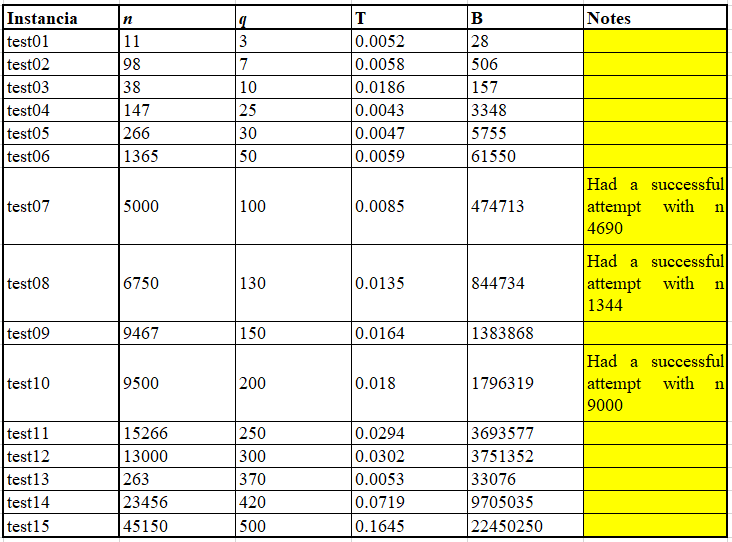
\includegraphics[width=130mm]{img/TablaDP.png}
			\begin{figure}[!]				
				\centering
				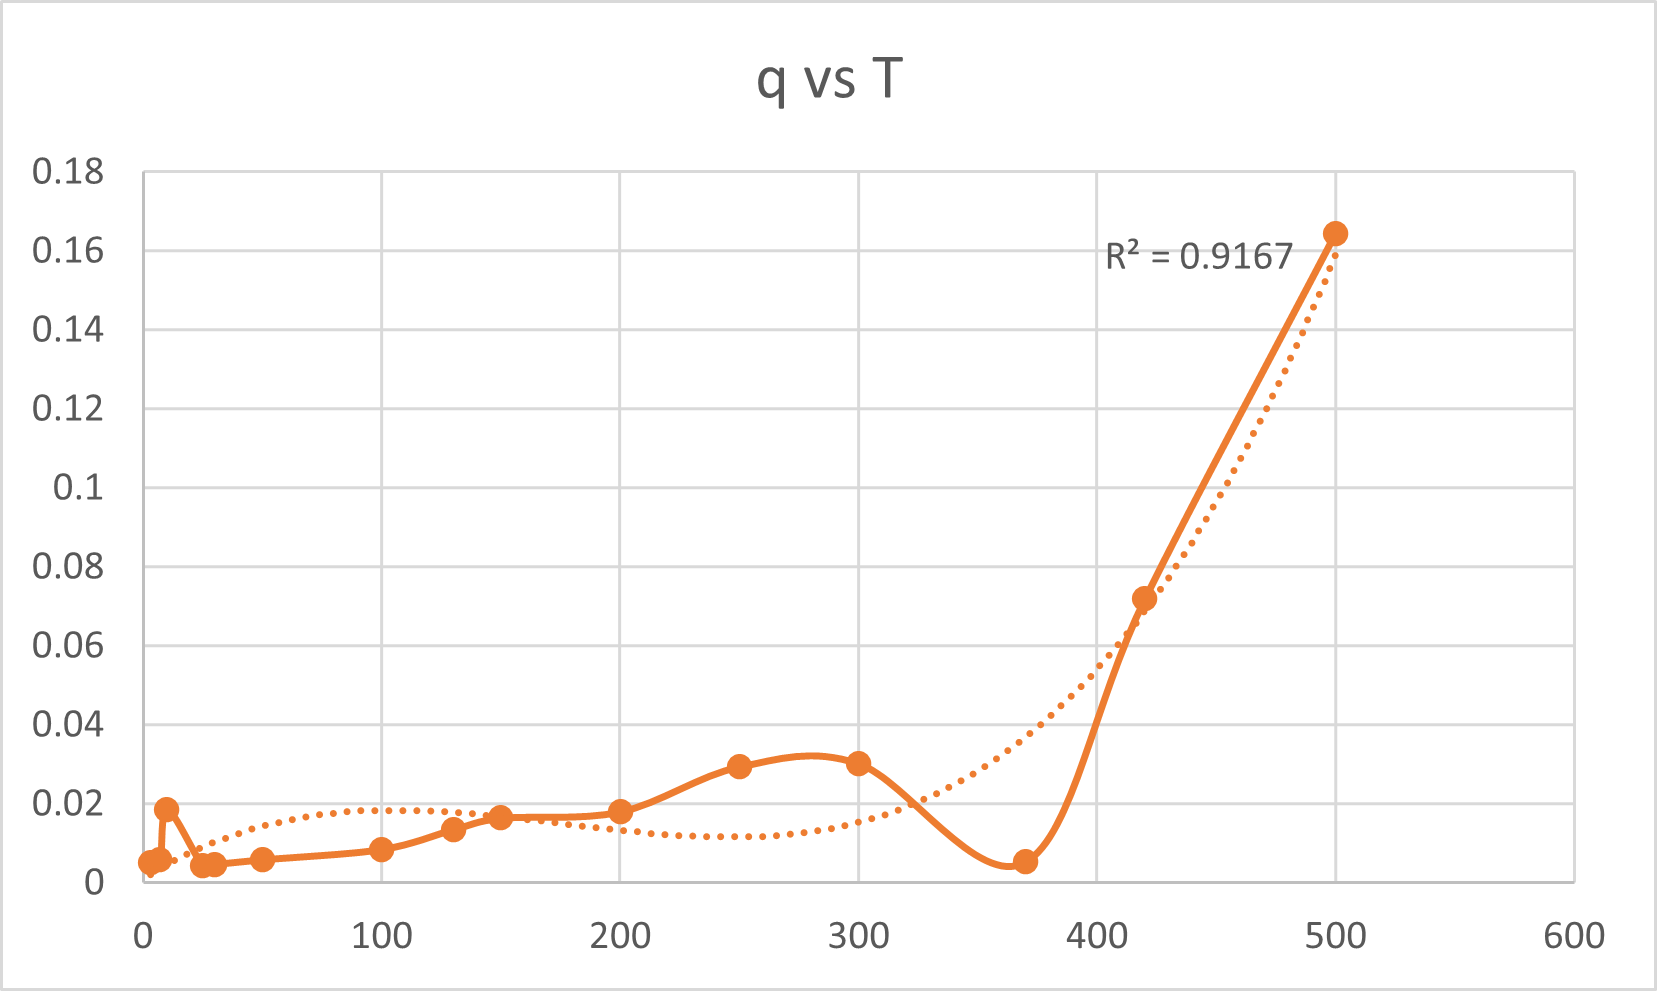
\includegraphics{img/DP_qvsT.png}
				\caption{$q$ vs $T$. Línea de tendencia polinómica clase 3; $y = 5E-09x^3 - 3E-06x^2 + 0.0004x + 0.0011
				$, $R^2 = 0.9167$}
			\end{figure}

			\begin{figure}[!]
				\centering
				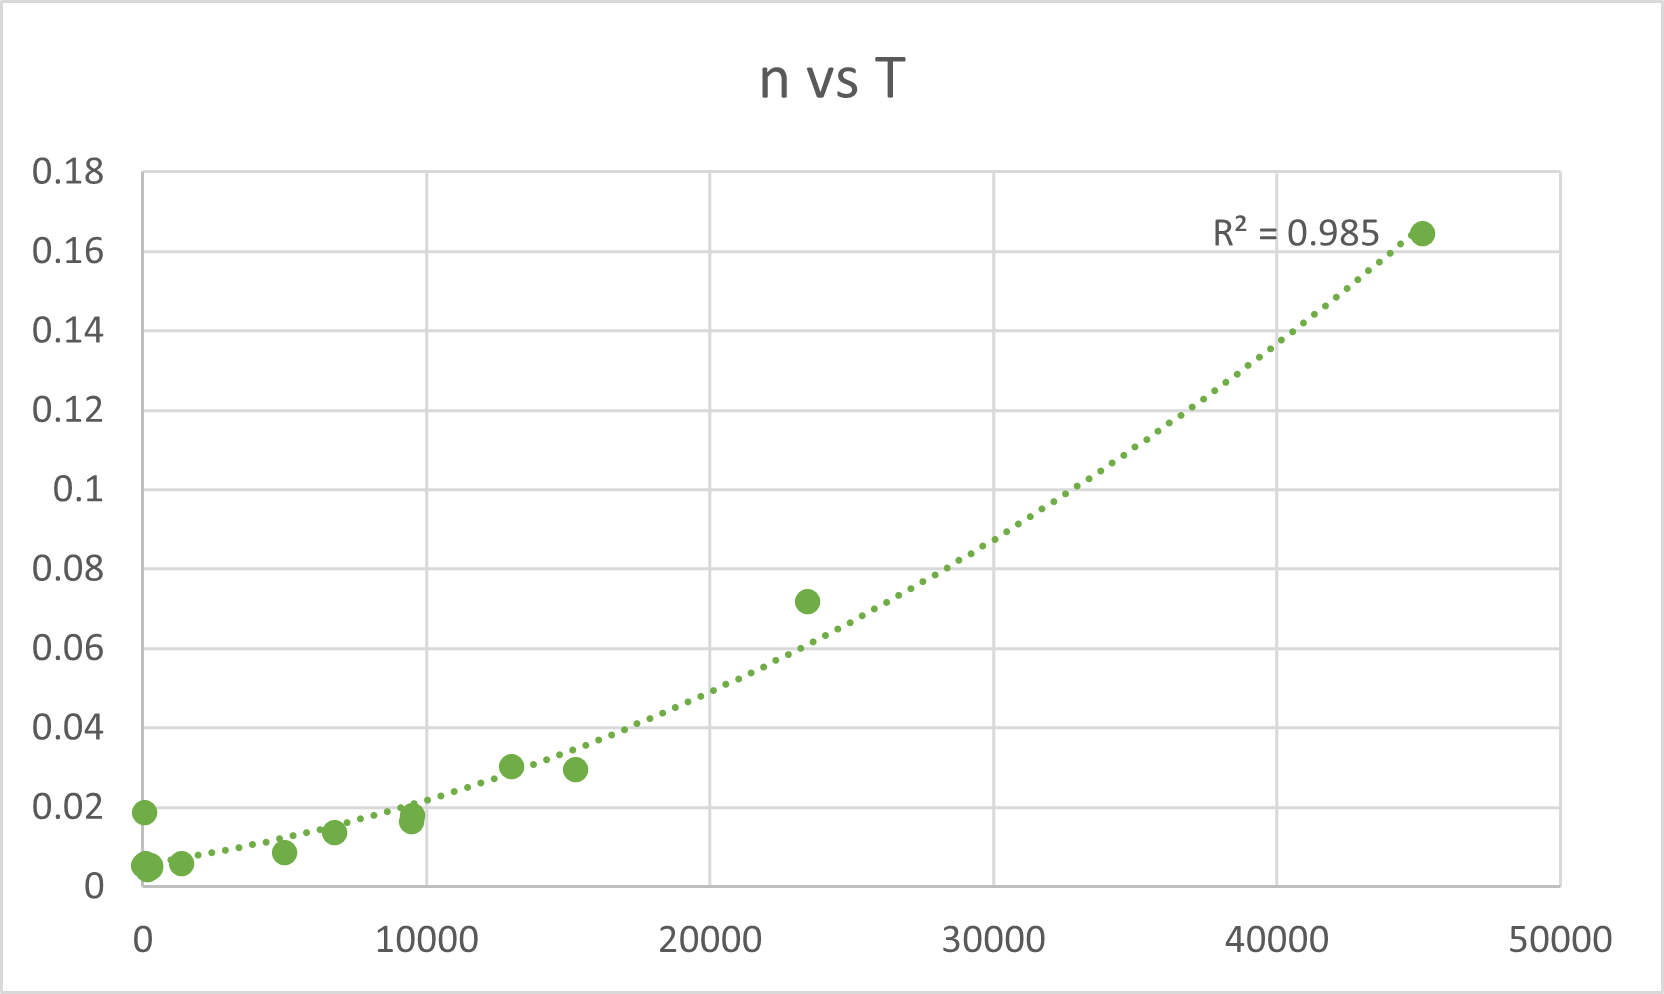
\includegraphics{img/DP_nvsT.png}
				\caption{$n$ vs $T$. Línea de tendencia polinómica clase 2; $y = 6E-11x^2 + 1E-06x + 0.0057$, $R^2 = 0.985$}
			\end{figure}
			
		\pagebreak
		\subsubsection{\underline{Análisis de resultados}}
			\par Es notable la enorme cantidad de operaciones que realiza este algoritmo conforme el tamaño de entrada de datos aumenta. Tomando esto en cuenta, el tiempo de ejecución es notablemente bajo en tamaños de entrada de menos de 130 datos, menor que los resultados del algoritmo Greedy aunque no por mucho, pero entradas mayores a dicho número su tiempo va creciendo exponencialmente (con una línea de tendencia polinómica).
	\subsection{Video demostración}
		\par Link al video de demostración del proyecto: https://youtu.be/-5Ckw4Ocauk \\
		
\section{Aportaciones}
\begin{tabular}{ |p{3cm}|p{10cm}| }
	\hline
	\multicolumn{2}{|c|}{Aportaciones} \\
	\hline
	Carlos & Investigación, documentación, pruebas de código\\
	\hline
	Bernardo & Planificación, desarrollo y depuración de códigos, pruebas de código, ejecuciones de algoritmos, tablas y análisis de resultados\\
	\hline
\end{tabular}
\section{Aprendizajes}
\begin{tabular}{ |p{2cm}|p{4cm}|p{4cm}|p{4cm}| }
	\hline
	\multicolumn{4}{|c|}{Aprendizajes} \\
	\hline
	& Aprendizaje del curso &	Lo que más le agradó &	Lo que no le agradó \\
	\hline
	Carlos & La variedad y la lógica detrás de algunos algoritmos muy interesantes. & Ciertos algoritmos y la disponibilidad y actitud del maestro. & Ver tantos algoritmos por encima, en vez de ver pocos de mayor importancia y profundizar.\\
	\hline
	Bernardo & Aprender la importancia de eficientar un algoritmo, y la lógica de varios ejemplos concretos.  & El orden y la organización de las clases, la flexibilidad y disponibilidad del profesor a todas horas.  & En ocasiones la falta de imágenes y ejemplos, y la tremenda dificultad de ciertas tareas tras poca práctica en las clases.\\
	\hline
\end{tabular}

\section{Conclusiones}
	
\section{Referencias bibliográficas}
	\par Rodriguez Eduardo, (2021). Técnicas para el diseño de algoritmos. Algoritmos voraces (greedy) Sesión 15, p 4.
	\par Rodriguez Eduardo, (2021). Técnicas para el diseño de algoritmos. Programación dinámica Sesión 14, p 3.
	\par Kozen, D. Zaks, S. (s.f) Optimal Bounds for the ChangeMaking Problem. Recuperado de: https://www.cs.cornell.edu/~kozen/Papers/change.pdf
	\par Khov, Try (2020). Solving Minimum Coin change. Recuperado de: https://trykv.medium.com/how-to-solve-minimum-coin-change-f96a758ccade
	\par Back To Back SWE (2019). The Change Making Problem - Fewest Coins To Make Change Dynamic Programming. Video from: \\https://www.youtube.com/watch?v=jgiZlGzXMBw

\section{Anexos}
	\subsection{Anexo 1}
		\par Tabla de tiempos de ejecución
		\par Programación dinámica\\
		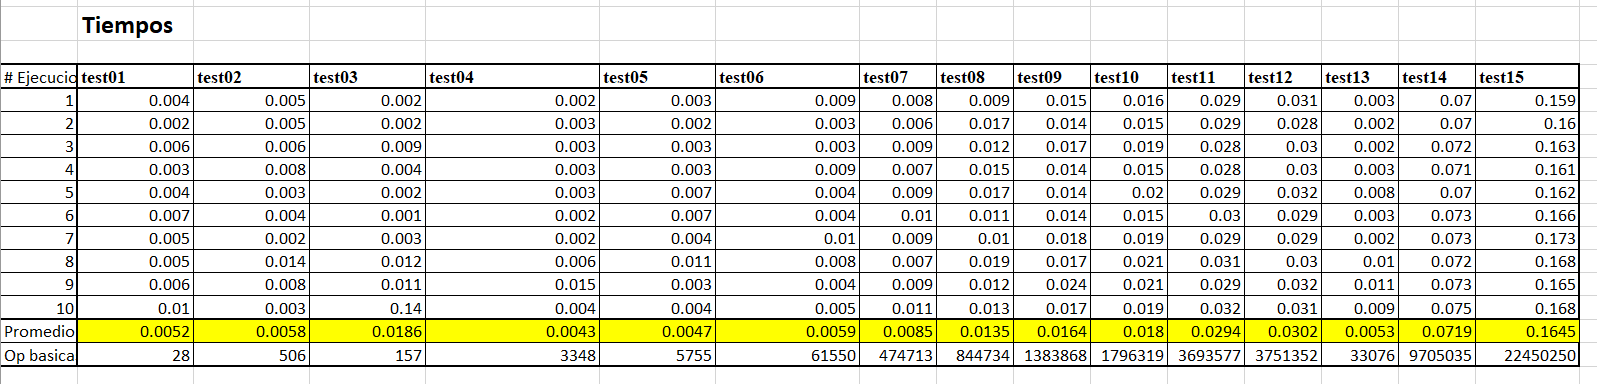
\includegraphics[width= 130mm]{img/TiemposDP.png}

% End of document
\end{document}